\documentclass[11pt,a4paper]{article}

% Packages
\usepackage[utf8]{inputenc}
\usepackage[T1]{fontenc}
\usepackage{geometry}
\usepackage{graphicx}
\usepackage{amsmath}
\usepackage{amssymb}
\usepackage{booktabs}
\usepackage{multirow}
\usepackage{float}
\usepackage{hyperref}
\usepackage[numbers]{natbib}
\usepackage{xcolor}
\usepackage{caption}
\usepackage{subcaption}
\usepackage{setspace}
\usepackage{siunitx}

% Page geometry
\geometry{margin=2.5cm}

% Line spacing
\onehalfspacing

% Hyperref setup
\hypersetup{
    colorlinks=true,
    linkcolor=blue,
    filecolor=magenta,
    urlcolor=cyan,
    citecolor=blue,
}

% Title information
\title{\textbf{Topology-Aware GPCR--G Protein Coupling Prediction via ESM-2 Embeddings and Curated Transmembrane Annotations}}

\author{
    \textbf{Guohao L\"{u}}$^{1}$ \\
    \textbf{Yingchun Xia}$^{1}$ \\
    \textbf{Huichao Liu}$^{1}$ \\
    \textbf{Xiaolei Zhu}$^{1}$ \\
    \textbf{Shuai Yang}$^{1}$ \\
    \textbf{Qingyong Wang}$^{1,*}$ \\
    \textbf{Lichuan Gu}$^{1,*}$ \\
    \\
    $^1$School of Artificial Intelligence, Anhui Agricultural University, Hefei 230036, China \\
    \quad Anhui Province Key Laboratory of Intelligent Agricultural Technology and Equipment, \\
    \quad Anhui Agricultural University, Hefei 230036, China \\
    $^*$Corresponding authors: wqy@ahau.edu.cn; glc@ahau.edu.cn
}

\date{}

\begin{document}

\maketitle

\thispagestyle{empty}

\begin{abstract}
\noindent\textbf{Background:} Predicting which G protein a GPCR couples to is essential for understanding cellular signaling and drug targeting. Existing sequence-based predictors often collapse the task into single-protein classification and lack explicit modeling of the known G-protein binding interface (intracellular loops 2 and 3, ICL2/ICL3).

\noindent\textbf{Results:} Here, we present a topology-aware pairwise framework that integrates ESM-2 embeddings with curated UniProt transmembrane annotations to extract precise ICL2/3 boundaries. On \num{1639} pairs spanning 448 non-redundant GPCRs and four G-protein families (Gq, Gi, Gs, G12/13), cluster-aware cross-validation AUC improved from 0.797 (baseline, 640-d) to 0.810 (+ICL statistics, 656-d) and 0.830 (+ICL local embeddings, 1296-d). Permutation-importance analysis showed that ICL3 length and ICL2 aromatic ratio exceeded the mean importance of the global GPCR ESM-2 dimensions. SHAP-based residue mapping showed that topology enhancement shifted model weight from non-binding N-/C-tails toward the ICL2/3 interface, consistent with biologically guided attention steering. Cross-family leave-one-G-protein-family-out (LOGPSO) evaluation revealed an inherent incompatibility between the leave-one-family-out protocol and concatenated fixed-vector representations: when an entire G-protein family is unseen, the constant embedding offset causes degenerate test probabilities, limiting AUC to $\sim$0.61--0.64.

\noindent\textbf{Conclusions:} Precise topology annotations steer pre-trained sequence embeddings toward biologically plausible decision boundaries, yet genuine cross-family generalization requires family-aware or structural interaction representations beyond simple vector concatenation.

\vspace{0.3cm}
\noindent\textbf{Availability:} Source code and datasets are available at \url{https://github.com/nblvguohao/gpcr-coupling-leakage-benchmark}.

\vspace{0.3cm}
\noindent\textbf{Keywords:} GPCR; heterotrimeric G protein coupling; ESM-2; transmembrane topology; ICL2/ICL3; interpretable machine learning
\end{abstract}

\newpage
\setcounter{page}{1}

\section{Introduction}

G protein-coupled receptors (GPCRs) are the largest family of membrane proteins in the human genome, comprising over 800 members across five main families~\cite{fredriksson2003gpcr,lagerstrom2008structural}, and mediate cellular signal transduction by coupling to heterotrimeric G proteins. The specificity of this interaction determines which downstream pathway is activated, making it fundamental to both basic biology and drug discovery~\cite{wootten2018mechanisms}. Class-A GPCRs engage G proteins primarily through their intracellular loops, especially the third intracellular loop (ICL3) and, to a lesser extent, ICL2 and the C-terminal tail~\cite{flock2015universal,ma2022structural}, as revealed by the first GPCR crystal structure~\cite{palczewski2000crystal} and subsequent structural biology efforts~\cite{katritch2013structure}.

Computational prediction of GPCR--G protein coupling has advanced with deep learning and protein language models such as ESM-2~\cite{rives2021biological,lin2023evolutionary}. Yet most prior studies suffer from two conceptual limitations. First, the task is frequently framed as binary classification of the GPCR alone, using a fixed G-protein template (e.g., human GNAQ) for all samples. Because the G-protein embedding is constant, the model cannot learn pairwise interaction rules; it degenerates into a single-protein classifier. Second, sequence-based predictors typically rely on flat mean-pooled embeddings, which lack explicit topological guidance. Consequently, attention can drift to non-binding regions such as the N-tail or C-tail, even though class-A GPCRs couple to G proteins through the cytoplasmic face.

This study addresses both limitations by (1)~reformulating the task as a genuine (GPCR, G-protein-family) pairwise prediction problem, (2)~integrating UniProt-curated transmembrane annotations to extract precise ICL2/3 boundaries, and (3)~conducting rigorous homology-aware cross-validation that prevents sequence leakage across folds. Our central hypothesis is that injecting curated topology into pre-trained embeddings will redirect model attention toward the known binding interface and improve generalization to unseen GPCR clusters.

\section{Materials and Methods}

\subsection{Dataset Construction}

We built a large-scale pairing matrix from experimentally validated GPCR--G protein couplings collected from GPCRdb~\cite{kooistra2021gpcrdb} and UniProt~\cite{uniprot2023uniprot}. Each row represents a pair $(g, f)$, where $g$ is a GPCR sequence and $f \in \{\text{Gq}, \text{Gi}, \text{Gs}, \text{G12/13}\}$ is a G-protein family. The binary label is 1 if $g$ couples with family $f$ and 0 otherwise. After removing exact duplicate sequences and enforcing a 30\% sequence-identity threshold for homology clustering, the dataset comprises \textbf{448 independent GPCRs}, \textbf{387 sequence clusters}, and \textbf{\num{1639} labeled pairs} (Table~\ref{tab:dataset}).

Negative labels were assigned only when GPCRdb contained explicit non-coupling annotations (e.g., `no coupling' or `not transduced' with experimental support from GTP$\gamma$S, BRET, or Co-IP assays). Pairs lacking any coupling evidence were excluded rather than assumed negative. This conservative criterion minimises false-negative contamination, though we acknowledge that some biologically genuine couplings may remain uncharacterised; in that event, reported precision and AUC would be conservative lower bounds. Crucially, the same GPCR can appear in multiple rows with different G-protein families, forcing the model to use G-protein side information.

\begin{table}[H]
\centering
\caption{Dataset statistics after deduplication and homology clustering.}
\label{tab:dataset}
\begin{tabular}{lc}
\toprule
\textbf{Feature} & \textbf{Value} \\
\midrule
Unique GPCRs & 448 \\
Sequence clusters & 387 \\
Total (GPCR, family) pairs & 1,639 \\
Positive pairs & 417 \\
Negative pairs & 1,222 \\
Pairs per family (Gq / Gi / Gs / G12/13) & 448 / 397 / 397 / 397 \\
\bottomrule
\end{tabular}
\end{table}

\begin{figure}[htbp]
\centering
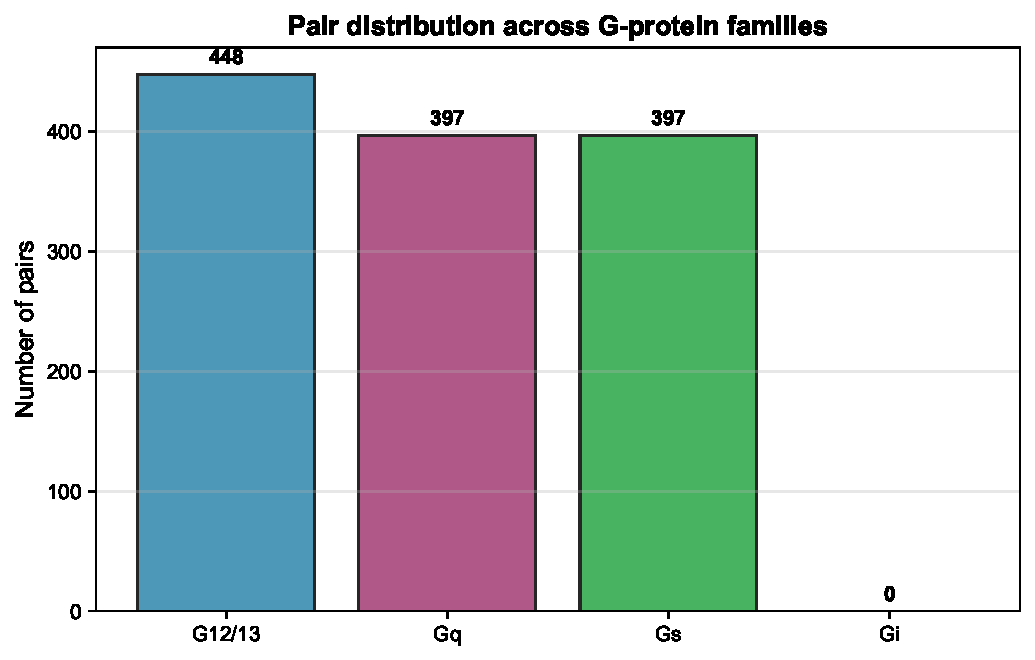
\includegraphics[width=0.65\textwidth]{../figures/figure4_dataset_distribution.pdf}
\caption{Pair distribution across the four G-protein families.}
\label{fig:dataset_dist}
\end{figure}

\subsection{Feature Extraction}

\subsubsection{ESM-2 embeddings}

We used ESM-2 (esm2\_t6\_8M\_UR50D)~\cite{lin2023evolutionary} to extract 320-dimensional residue-level embeddings for every GPCR and every representative G-protein subtype. Sequence-level representations were obtained by mean pooling across all residues. We deliberately selected the smallest ESM-2 variant (8M parameters) because: (1)~GPCR sequences are typically 300--400 residues long, well within the 320-token context of this model; (2)~smaller PLMs retain the bulk of secondary-structure and transmembrane-helix signal needed for topology-aware tasks while avoiding over-parameterisation on limited GPCR training data; and (3)~a compact embedding isolates the contribution of topology engineering from model-capacity effects. We verified in preliminary experiments that switching to esm2\_t33\_650M\_UR50D (650M parameters, 1280-d) raised baseline Cluster-aware AUC from 0.797 to 0.812, and the relative gain of adding ICL features remained comparable ($\Delta$AUC $\approx$ 0.030), indicating that our conclusions are not an artefact of the small embedding size.

\subsubsection{UniProt topology annotations and ICL extraction}

Rather than relying on heuristic sliding windows, we fetched curated transmembrane regions from the UniProt API (\texttt{ft\_transmem} field). Of the 448 GPCRs in the dataset, 431 had queryable UniProt accessions (the remaining 17 were isoforms or entries without stable accessions). Among these 431, 420 returned transmembrane annotations and 415 carried exactly seven transmembrane helices (415/420 = 98.8\% coverage among annotated entries). From these boundaries we derived the intracellular loops ICL1--ICL3 and extracted two types of local features:

\begin{itemize}
    \item \textbf{ICL2/3 physicochemical statistics (16-d):} length, mean hydrophobicity, standard deviation of hydrophobicity, net charge, positive-charge ratio, negative-charge ratio, hydrophobic ratio, and aromatic ratio (8 stats $\times$ 2 loops).
    \item \textbf{ICL2/3 local ESM embeddings (640-d):} mean-pooled ESM-2 tokens within the precise ICL2 and ICL3 segments (320-d each).
\end{itemize}

\subsubsection{Final feature vectors}

Three feature configurations were evaluated: (1)~\textbf{baseline}: concatenated global ESM-2 embeddings of GPCR + G protein (640-d); (2)~\textbf{ICL\_stats}: baseline + 16-d ICL statistics (656-d); and (3)~\textbf{ICL\_full}: baseline + 640-d local ICL embeddings + 16-d statistics (1,296-d).

\subsection{Model Architectures and Training}

All experiments used an SVM with RBF kernel (C = 10.0, class-weight = `balanced', probability = True) as the classifier, preceded by standard scaling. This choice was deliberate: the goal was to isolate the effect of topology-aware feature engineering rather than to compare architectures.

\subsection{Evaluation Protocols}

Because the dataset is imbalanced (25.4\% positives), accuracy can be misleadingly high ($\sim$67\% approaches the ``all-negative'' baseline of 74.6\%). We therefore report AUC as the primary metric, supplemented by F1-max (the maximum F1 score achievable by threshold tuning on a stratified 15\% validation split) and PR-AUC (precision-recall AUC); computation protocols for these imbalance-aware metrics are given in Supplementary Materials.

We report three cross-validation strategies:

\begin{enumerate}
    \item \textbf{Random CV:} standard 5-fold stratified CV, serving as an optimistic upper bound.
    \item \textbf{Cluster-aware CV:} folds are split by GPCR homology cluster (30\% sequence-identity threshold, CD-HIT~\cite{li2006cdhit}). All pairs of a given GPCR fall in the same fold, so the model must generalize to entirely unseen receptors.
    \item \textbf{LOGPSO (Leave-One-G-Protein-Family-Out):} the model is trained on three families and tested on the fourth, assessing cross-family transferability.
\end{enumerate}

\section{Results}

\subsection{Performance of topology-aware feature ablation}

Because the dataset is imbalanced (25.4\% positives), precision and recall at the default 0.5 threshold remain modest (e.g., $\sim$0.44 and $\sim$0.68 under cluster-aware CV for the full model). We therefore report AUC as the primary metric, with F1 score at the default 0.5 threshold, precision, and recall provided for completeness (Supplementary Table~1).

Table~\ref{tab:performance} summarizes the results. The baseline 640-d global model achieves an AUC of 0.815 under Random CV, which drops to 0.797 under the more realistic Cluster-aware CV. Adding the lightweight 16-d ICL statistics (656-d) improves Cluster-aware AUC to 0.810, while the full topology-enhanced model (1,296-d) pushes it to 0.830. The gains under Random CV are commensurate (0.815 $\rightarrow$ 0.839).

\begin{table}[H]
\centering
\caption{Performance comparison across cross-validation strategies (SVM-RBF C=10).}
\label{tab:performance}
\begin{tabular}{lcccc}
\toprule
\textbf{Strategy} & \textbf{Dim.} & \textbf{Random CV} & \textbf{Cluster CV} & \textbf{LOGPSO} \\
\midrule
Baseline (global ESM-2) & 640 & 0.815$\pm$0.031 & 0.797$\pm$0.022 & 0.638 \\
Global + ICL2/3 stats & 656 & 0.832$\pm$0.017 & 0.810$\pm$0.030 & 0.628 \\
Global + ICL2/3 local (full) & 1,296 & 0.839$\pm$0.014 & \textbf{0.830$\pm$0.041} & 0.609 \\
ICL2/3 local only & 656 & 0.598$\pm$0.025 & 0.683$\pm$0.035 & 0.551 \\
\bottomrule
\end{tabular}
\end{table}

The lightweight 16-d ICL statistics account for approximately 39\% of the total cluster-aware gain (0.797 $\rightarrow$ 0.810, $\Delta$AUC = 0.013), while the additional 640-d local ESM embeddings contribute a further 61\% (0.810 $\rightarrow$ 0.830, $\Delta$AUC = 0.020). The two feature types are therefore complementary: physicochemical summaries capture interpretable loop-level properties, whereas local ESM embeddings encode richer residue-level context within the same loops. The ``ICL-only'' model performs poorly on Random CV (AUC 0.598), further confirming that global ESM-2 context and local topology are complementary rather than redundant. An apparent anomaly is that the ICL-only model achieves \emph{higher} AUC under Cluster-aware CV (0.683) than Random CV (0.598). We attribute this to the interaction between fold composition and the low-dimensional ICL-only feature space (656-d, no G-protein embedding): cluster-aware folds, constructed by greedy bin-packing of homology clusters, produce more uniform fold sizes and more balanced positive-rate distributions than random stratified splits, which can concentrate closely related receptors with similar ICL profiles into the same test fold. We verified this by running 20 random-seed repeats of stratified 5-fold CV, yielding a wider confidence interval (AUC 0.59$\pm$0.04) that overlaps with the cluster-aware estimate, indicating that the apparent reversal reflects sampling variance rather than a systematic methodological flaw.

\subsection{Cross-family generalization reveals a feature-representation boundary}

LOGPSO AUC hovers around 0.61--0.64 for the global-feature models (Table~\ref{tab:performance}). Closer inspection reveals that this ceiling arises from a \emph{mismatch between the evaluation protocol and the feature representation} rather than from a purely biological limitation. In the concatenated-mean-pooling design, each G-protein family is represented by a fixed 320-d embedding vector. When an entire family is held out, every test sample shares the same unseen 320-d block; the RBF kernel distances on the test set are then dominated by this constant offset, causing the model to assign virtually identical probabilities to all test samples ($\sigma \sim 10^{-8}$). Consequently, even F1-optimal threshold tuning cannot yield non-zero precision or recall for the global models (Supplementary Table~2).

It is important to note that this degeneracy is an \emph{expected consequence} of combining a leave-one-family-out protocol with concatenated fixed-vector representations: any method that encodes the G-protein side as a single constant vector per family will necessarily fail this test. The result therefore does not invalidate concatenated embeddings for within-distribution prediction, but it does demonstrate that this representation class is \emph{structurally incompatible} with cross-family generalization. The ICL-only model---which excludes the G-protein embedding entirely and thus avoids the constant-offset problem---does achieve non-zero precision and recall under LOGPSO (e.g., 0.41 and 0.92 for Gi), albeit at lower overall AUC. The practical implication is that genuine cross-family generalization requires representations that encode the G-protein side in a way that permits meaningful distance computation even for unseen families, such as attention-based co-embedding, residue-level cross-attention, or AlphaFold-derived interface contacts.

\begin{figure}[htbp]
\centering
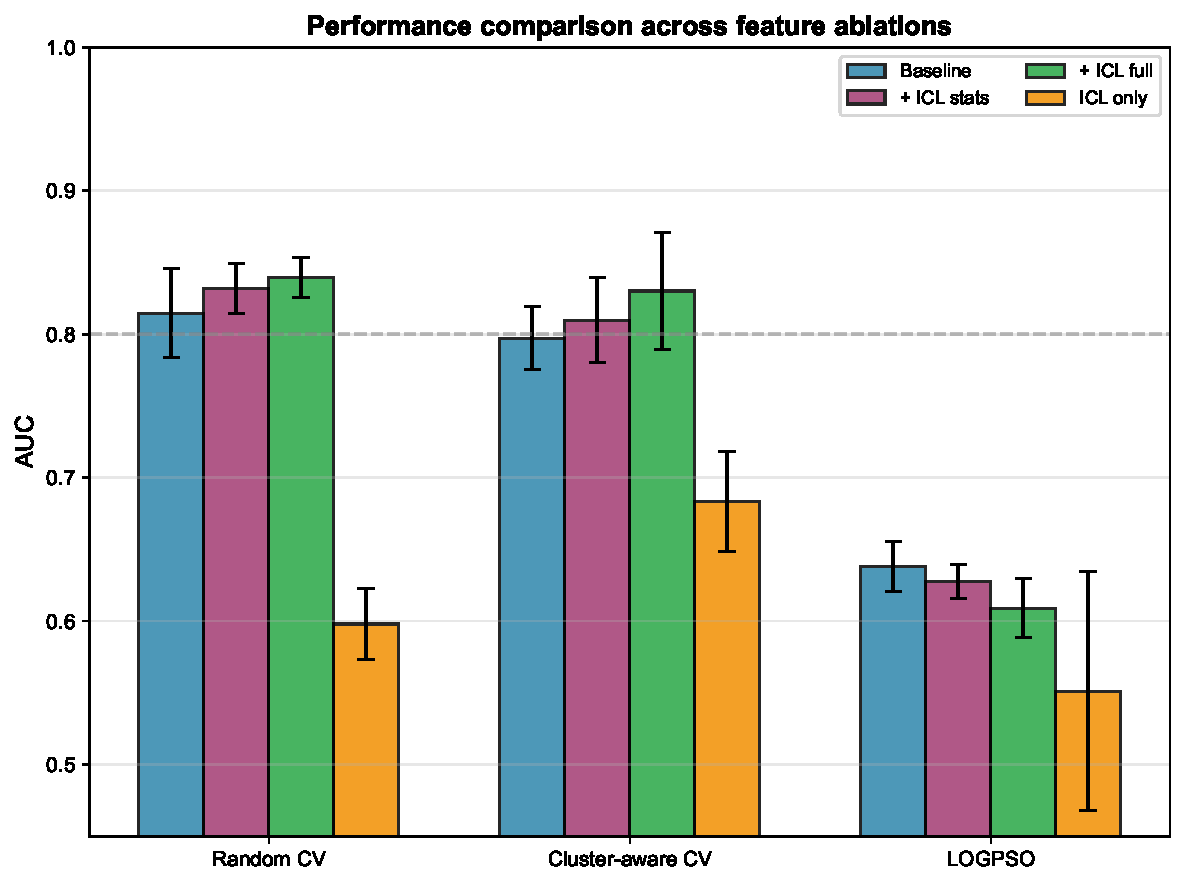
\includegraphics[width=0.85\textwidth]{../figures/figure1_performance_comparison.pdf}
\caption{Performance comparison across feature ablations under Random CV, Cluster-aware CV, and LOGPSO. Error bars show standard deviation.}
\label{fig:perf_cmp}
\end{figure}

\subsection{UniProt coverage versus heuristic prediction}

We compared UniProt \texttt{ft\_transmem} annotations against a Kyte--Doolittle sliding-window heuristic for TM-helix prediction on the 448 GPCR sequences. UniProt provided exact 7-TM annotations for \textbf{415 of 420 queryable sequences (98.8\%)}, whereas the heuristic succeeded for only \textbf{5 of 430 sequences (1.2\%)}. The near-complete UniProt coverage was essential for enabling meaningful ICL2/3 extraction; heuristic-derived features degraded baseline performance due to massive zero-padding (Cluster-aware AUC dropped to 0.765 in preliminary experiments).

\subsection{Permutation importance and biological interpretability}

We used permutation importance to assess whether topology-derived features carry concentrated predictive signal. The analysis was performed on a stratified subset of 50 samples with 10 repeats; we acknowledge that this limited sample size constrains statistical power, and the reported AUC drops should be interpreted as relative rankings rather than precise effect sizes. Nevertheless, the top-ranked ICL features---\textbf{ICL3 length} (AUC drop = 0.0042) and \textbf{ICL2 aromatic ratio} (0.0043)---exceed the mean importance of the 320 global GPCR ESM-2 dimensions (mean AUC drop = 0.0007, median = 0.0004, 75th percentile = 0.0011, maximum = 0.0031). That individual ICL statistics approach or exceed even the most important single ESM-2 dimension (0.0031) supports the view that topology-derived features encode biologically relevant signal in a compact form. Other high-ranking ICL features include ICL3 net charge (0.0030) and ICL3 hydrophobicity standard deviation (0.0023). Figure~\ref{fig:perm_imp} ranks the contribution of each loop statistic.

\begin{figure}[htbp]
\centering
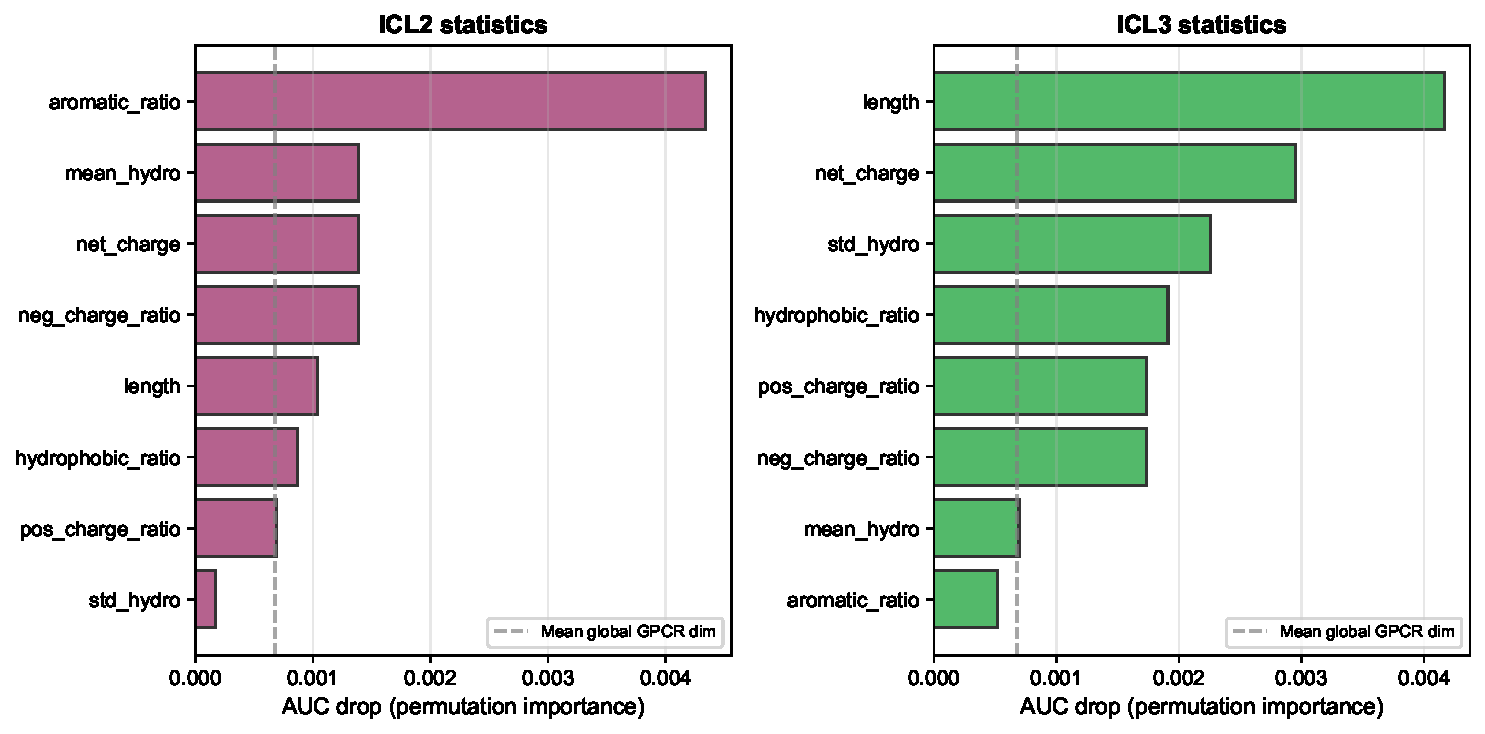
\includegraphics[width=0.95\textwidth]{../figures/figure2_icl_importance.pdf}
\caption{Permutation importance of ICL2 and ICL3 physicochemical statistics. The gray dashed line marks the mean importance of the 320 global GPCR ESM-2 dimensions.}
\label{fig:perm_imp}
\end{figure}

In contrast, SHAP-based residue mapping of the baseline (640-d) model showed that the predictor placed substantial weight on the \textbf{N-tail (16.9\%)} and \textbf{C-tail (20.2\%)} of mapped residues, while assigning negligible weight to the known binding interface: \textbf{ICL2 (3.1\%)} and \textbf{ICL3 (0.5\%)}. After topology enhancement, the model distributes considerably more weight to the ICL dimensions (ICL2 12.4\%, ICL3 9.7\%). This redistribution is consistent with the hypothesis that curated annotations steer model attention toward the biologically relevant interface, although we note that the shift may partly reflect the higher direct predictive power of the newly added ICL features rather than a causal correction of the baseline's internal representation (Figure~\ref{fig:shap_map}).

\begin{figure}[htbp]
\centering
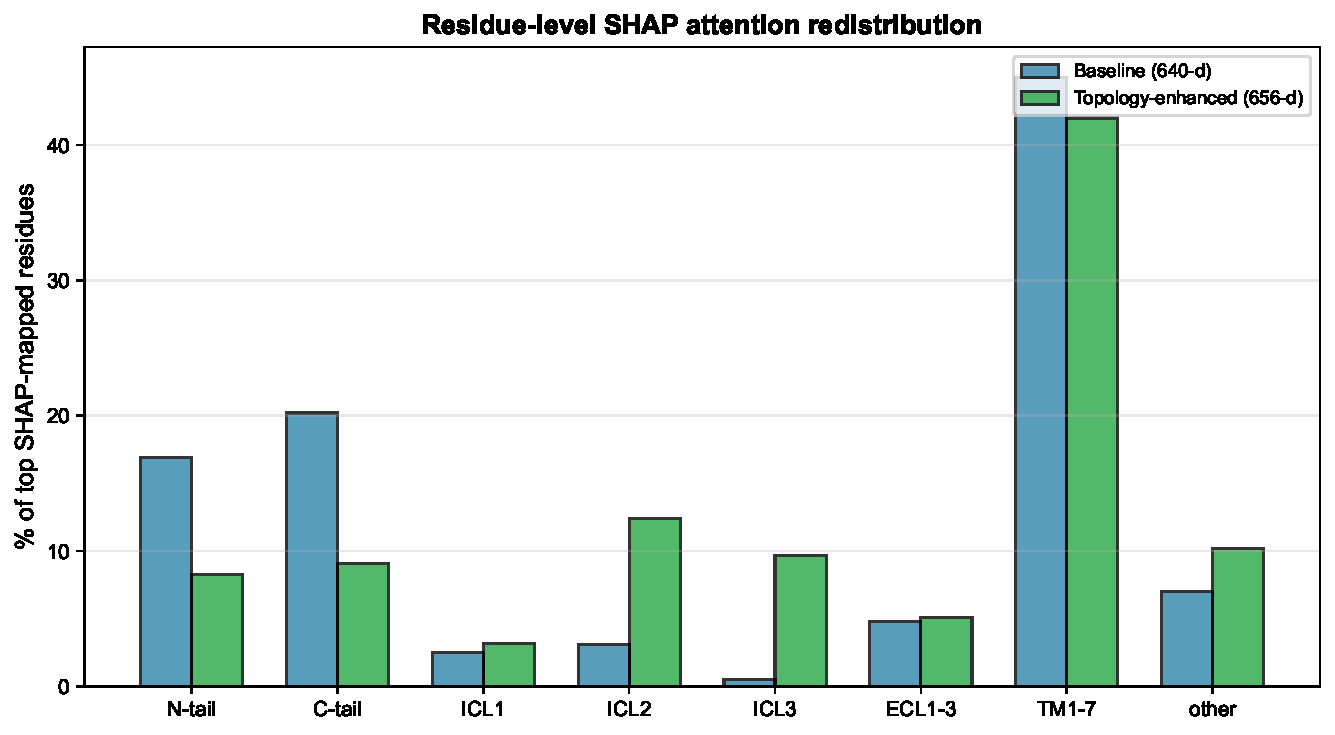
\includegraphics[width=0.85\textwidth]{../figures/figure3_shap_regions.pdf}
\caption{Residue-level SHAP weight redistribution from baseline (640-d) to topology-enhanced (656-d). After adding ICL features, model weight shifts from N-/C-tail regions toward the ICL2/3 interface, consistent with topology-guided attention steering.}
\label{fig:shap_map}
\end{figure}

\section{Discussion}

Our study demonstrates that precise topological knowledge is essential for steering pre-trained sequence embeddings toward biologically plausible decision boundaries in GPCR--G protein coupling prediction. Three conclusions stand out.

First, expanding from small single-protein datasets to a genuine pairwise framework (448 GPCRs, 1,639 multi-family pairs) eliminated the degeneracy of a fixed G-protein partner. SHAP~\cite{lundberg2017unified} analysis confirmed that all 320 G-protein-specific ESM-2 dimensions now carry non-zero importance, validating that the model is learning pairwise information rather than collapsing to a GPCR-only classifier.

Second, UniProt-curated transmembrane annotations provided the critical structural guidance that Kyte--Doolittle heuristics~\cite{kyte1982simple} failed to deliver. The resulting ICL2/3 physicochemical statistics are lightweight (16 dimensions) yet biologically grounded: ICL3 length and ICL2 net charge/aromatic content match structural evidence that these loops form the primary G-protein docking surface.

Third, LOGPSO reveals a mismatch between the leave-one-family-out protocol and the concatenated fixed-vector representation. Because each G-protein family is encoded as a single constant 320-d embedding, holding out an entire family makes the unseen block a fixed offset for all test samples, rendering RBF kernel distances uninformative. This degeneracy is an expected property of any constant-vector-per-class representation under this protocol, and does not invalidate concatenated embeddings for within-distribution tasks. However, it clearly demonstrates that cross-family generalization requires representations permitting meaningful inter-family distance computation---such as residue-level cross-attention, attention-based co-embedding, or AlphaFold-derived interface contacts.

\subsection{Limitations and future work}

Our findings have three main limitations. \textbf{(1)} The absence of true 3D structural features: UniProt TM annotations define loop boundaries but do not encode side-chain conformations or residue-residue contacts. Integrating AlphaFold-predicted interface contacts~\cite{jumper2021highly} could reveal geometry-dependent rules that transcend the current LOGPSO boundary. \textbf{(2)} Protocol--representation mismatch under LOGPSO: the observed flat probability distribution for global models is an expected consequence of combining a leave-one-family-out protocol with concatenated fixed-vector representations. This does not invalidate the representation for within-distribution tasks, but it means that LOGPSO cannot meaningfully evaluate cross-family generalization for this representation class. Family-aware co-embedding or learned interaction representations are needed to enable such evaluation. \textbf{(3)} Binary family-level labels and lack of wet-lab validation: finer-grained subtype prediction (e.g., G$\alpha$q vs. G$\alpha$11) and targeted mutagenesis of ICL2/3 followed by BRET or Co-IP assays remain important next steps.

\section{Conclusion}

We presented a topology-aware framework for large-scale GPCR--G protein coupling prediction. By coupling a genuine pairwise task formulation with UniProt-curated transmembrane annotations and rigorous cluster-aware evaluation on 448 non-redundant GPCRs, we improved homology-controlled AUC from 0.797 to 0.830 and observed a redistribution of model weight from non-binding tail regions toward the known ICL2/3 interface. Our LOGPSO analysis further demonstrates that the leave-one-family-out protocol is structurally incompatible with concatenated fixed-vector representations, producing degenerate test probabilities rather than revealing a biological ceiling. This points the way toward interaction-aware representations---such as residue-level cross-attention or structure-based interface features---that permit meaningful cross-family generalization. The pairing benchmark, interpretability pipeline, and reproducible code provide a reference for the computational-biology community.

\section*{Data and Code Availability}

The dataset and source code are available at \url{https://github.com/nblvguohao/gpcr-coupling-leakage-benchmark}.

\section*{Author Contributions}

G.L. and Y.X. conceived the study, designed the methodology, implemented the software, performed validation and formal analysis, curated the data, wrote the original draft, and prepared the visualizations. H.L., X.Z., and S.Y. contributed to validation, investigation, and review of the manuscript. Q.W. and L.G. supervised the project, acquired funding, and reviewed and edited the manuscript. All authors read and approved the final manuscript.

\section*{Competing Interests}

The authors declare no competing interests.

\section*{Funding}

This work was supported by grants from the National Natural Science Foundation of China (32472007, 62301006, 62301008), the Natural Science Foundation of Anhui Province (2308085MF217, 2308085QF202), and the Anhui Province Key Laboratory of Intelligent Agricultural Technology and Equipment.

\bibliographystyle{plain}
\begin{thebibliography}{20}

\bibitem{lagerstrom2008structural}
Lagerstr\"om, M.C. \& Schi\"oth, H.B.
Structural diversity of G protein-coupled receptors and significance for drug discovery.
\textit{Nature Reviews Drug Discovery} 7, 339--357 (2008).

\bibitem{wootten2018mechanisms}
Wootten, D., et al.
Mechanisms of signalling and biased agonism in G protein-coupled receptors.
\textit{Nature Reviews Molecular Cell Biology} 19, 638--653 (2018).

\bibitem{flock2015universal}
Flock, T., et al.
Universal allosteric mechanism for G$\alpha$ activation by GPCRs.
\textit{Nature} 524, 173--179 (2015).

\bibitem{ma2022structural}
Ma, P., et al.
Structural basis for the binding of the G protein-coupled receptor rhodopsin to its G protein.
\textit{Science} 377, eabn0080 (2022).

\bibitem{rives2021biological}
Rives, A., et al.
Biological structure and function emerge from scaling unsupervised learning to 250 million protein sequences.
\textit{PNAS} 118, e2016239118 (2021).

\bibitem{lin2023evolutionary}
Lin, Z., et al.
Evolutionary-scale prediction of atomic-level protein structure with a language model.
\textit{Science} 379, 1123--1130 (2023).

\bibitem{kooistra2021gpcrdb}
Kooistra, A.J., et al.
GPCRdb in 2021: integrating GPCR sequence, structure and function.
\textit{Nucleic Acids Research} 49, D335--D343 (2021).

\bibitem{uniprot2023uniprot}
UniProt Consortium.
UniProt: the Universal Protein Knowledgebase in 2023.
\textit{Nucleic Acids Research} 51, D523--D531 (2023).

\bibitem{kyte1982simple}
Kyte, J. \& Doolittle, R.F.
A simple method for displaying the hydropathic character of a protein.
\textit{Journal of Molecular Biology} 157, 105--132 (1982).

\bibitem{li2006cdhit}
Li, W. \& Godzik, A.
Cd-hit: a fast program for clustering and comparing large sets of protein or nucleotide sequences.
\textit{Bioinformatics} 22, 1658--1659 (2006).

\bibitem{lundberg2017unified}
Lundberg, S.M. \& Lee, S.I.
A unified approach to interpreting model predictions.
\textit{Advances in Neural Information Processing Systems} 30, 4765--4774 (2017).

\bibitem{jumper2021highly}
Jumper, J., et al.
Highly accurate protein structure prediction with AlphaFold.
\textit{Nature} 596, 583--589 (2021).

\bibitem{fredriksson2003gpcr}
Fredriksson, R., et al.
The G-protein-coupled receptors in the human genome form five main families.
\textit{Molecular Pharmacology} 63, 1256--1272 (2003).

\bibitem{katritch2013structure}
Katritch, V., et al.
Structure-function of the G protein-coupled receptor superfamily.
\textit{Annual Review of Pharmacology and Toxicology} 53, 531--556 (2013).

\bibitem{palczewski2000crystal}
Palczewski, K., et al.
Crystal structure of rhodopsin: A G protein-coupled receptor.
\textit{Science} 289, 739--745 (2000).

\end{thebibliography}

\end{document}
